	\chapter{Results}\label{cha:results}
	Text
	
		\section{1D geological reservoir model results}
	
			\subsection{Scoring}
			\begin{figure}[h]
				\centering
				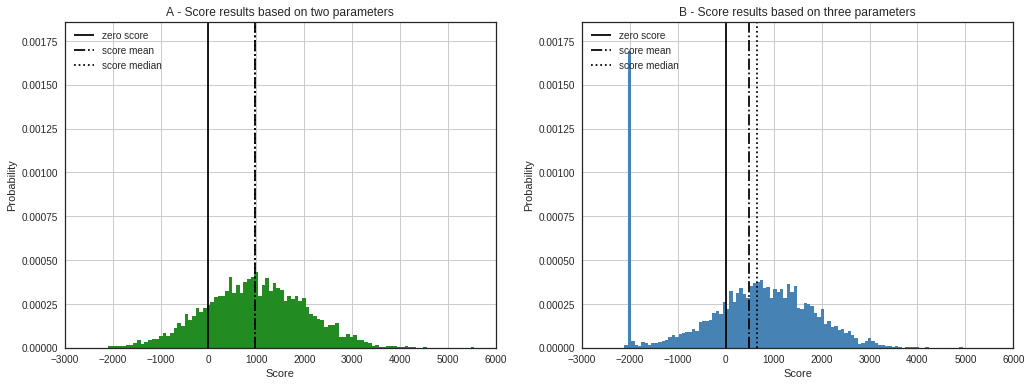
\includegraphics[width=1\textwidth]{Figures/score_results1.png}
				\caption{Posterior probability distributions from modeling scores using two (A) and three parameters (B).}\label{fig:score_results1}
			\end{figure}
			Results from scoring based on a 1D model constructed as defined in Section \ref{sec:1D_construction} are plotted in Figure \ref{fig:score_results1}. A test run of scoring with only the two parameters reservoir thickness and depth, is shown in \ref{fig:score_results1}-A. These results represented by an approximately normal distribution. The score is negative in about 17\% of the cases. Mean and median are about the same.\\	
			Full scoring results, including also seal reliability as a parameter, are visualized in Figure \ref{fig:score_results1}-B. The main distribution is not changed significantly, except for a striking peak of probability at the possibility for a score of -2000. This presumably represents the bulk of cases, in which the seal was assumed to have failed. It is to be noted, that the mean of the seal top distribution is found at -2000 m. It can be seen in Figure \ref{fig:1D_model}, that around that depth in the model column, reservoir top and seal top probability distributions significantly overlap. Thus, there is a possibility for a higher score, due to a shallower reservoir top position, but also a high probability for a seal that is to thin to be reliable. The negative score peak at -2000 is thus presumably caused by a high number of seal failures, due to both layer tops found in this area. Furthermore, mean and median of the score distribution have been shifted to lower values and are now found further apart.
			
			\subsection{Applying the custom loss function on the 1D reservoir scores}

			\begin{figure}[p!]
				\centering
				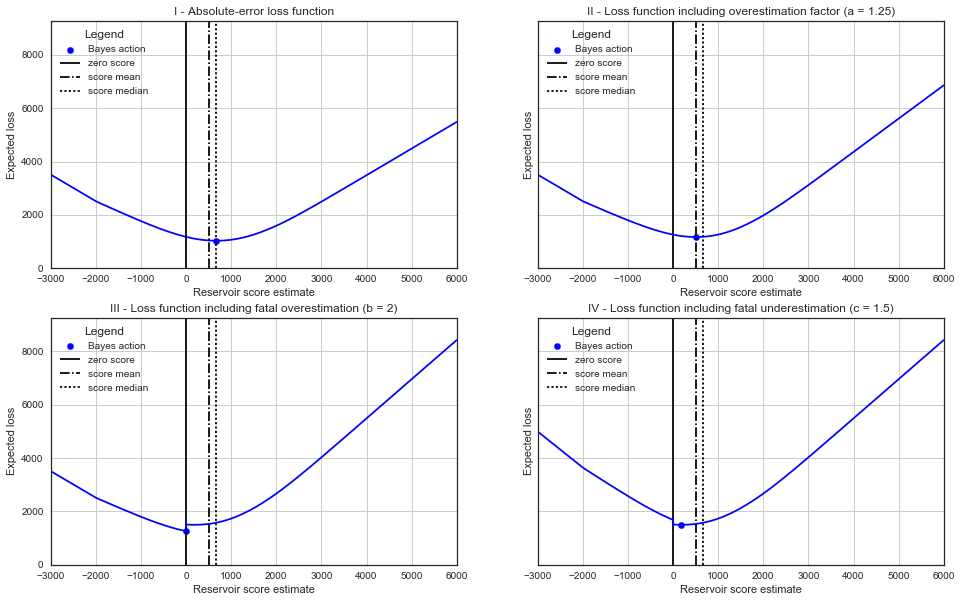
\includegraphics[width=1\textwidth]{Figures/LF_4steps.png}
				\caption{The single steps of customizing the loss function are depicted in plots I to IV.}\label{fig:LF_4steps}
				\centering
				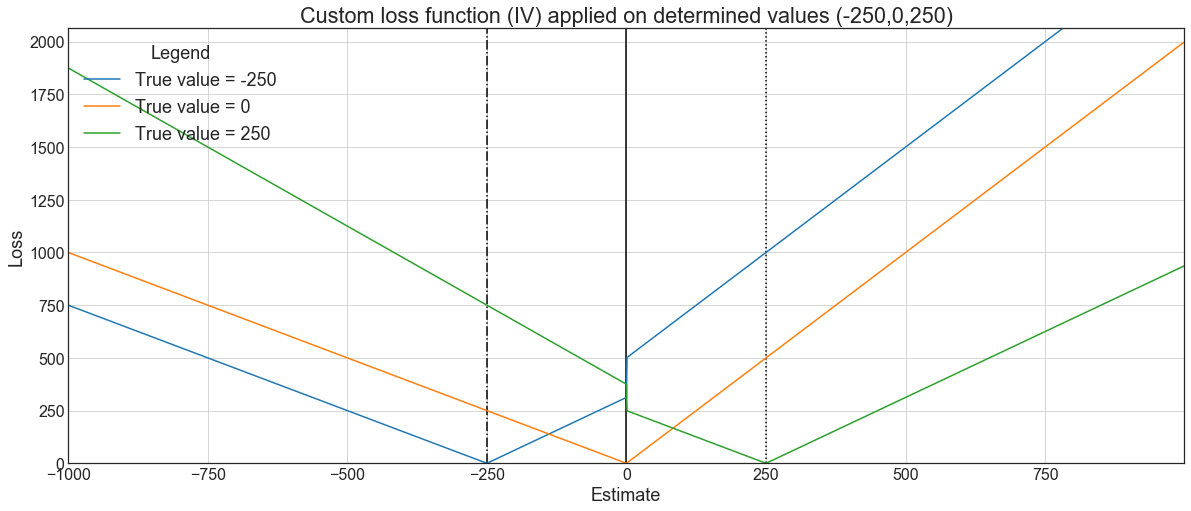
\includegraphics[width=1\textwidth]{Figures/LF4_det_values.png}
				\caption{Loss based on the customized loss function (Equation \ref{eq:LF_final}) for determined true scores of -750, 0 and 750.}\label{fig:LF4_det_values}
			\end{figure}			
			\begin{figure}[p!]
				\centering
				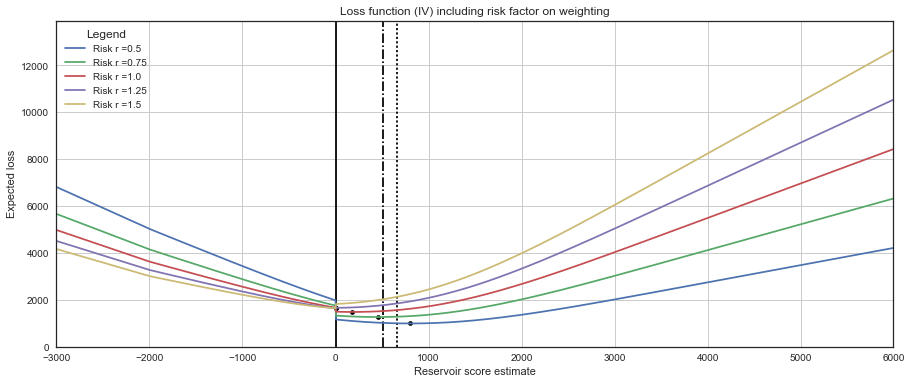
\includegraphics[width=1\textwidth]{Figures/LFR.png}
				\caption{Plotting of expected loss realizations after including the risk factor $r$ in the loss function (Equation \ref{eq:LFR_final}) for actors with risk-affinities ranging from risk-averse ($r$ = 0.5 and 0.75), over risk-neutral ($r$ = 1), to risk-friendly ($r$ = 1.25 and $r$ = 1.5).}\label{fig:1D_LFR} 
				\centering
				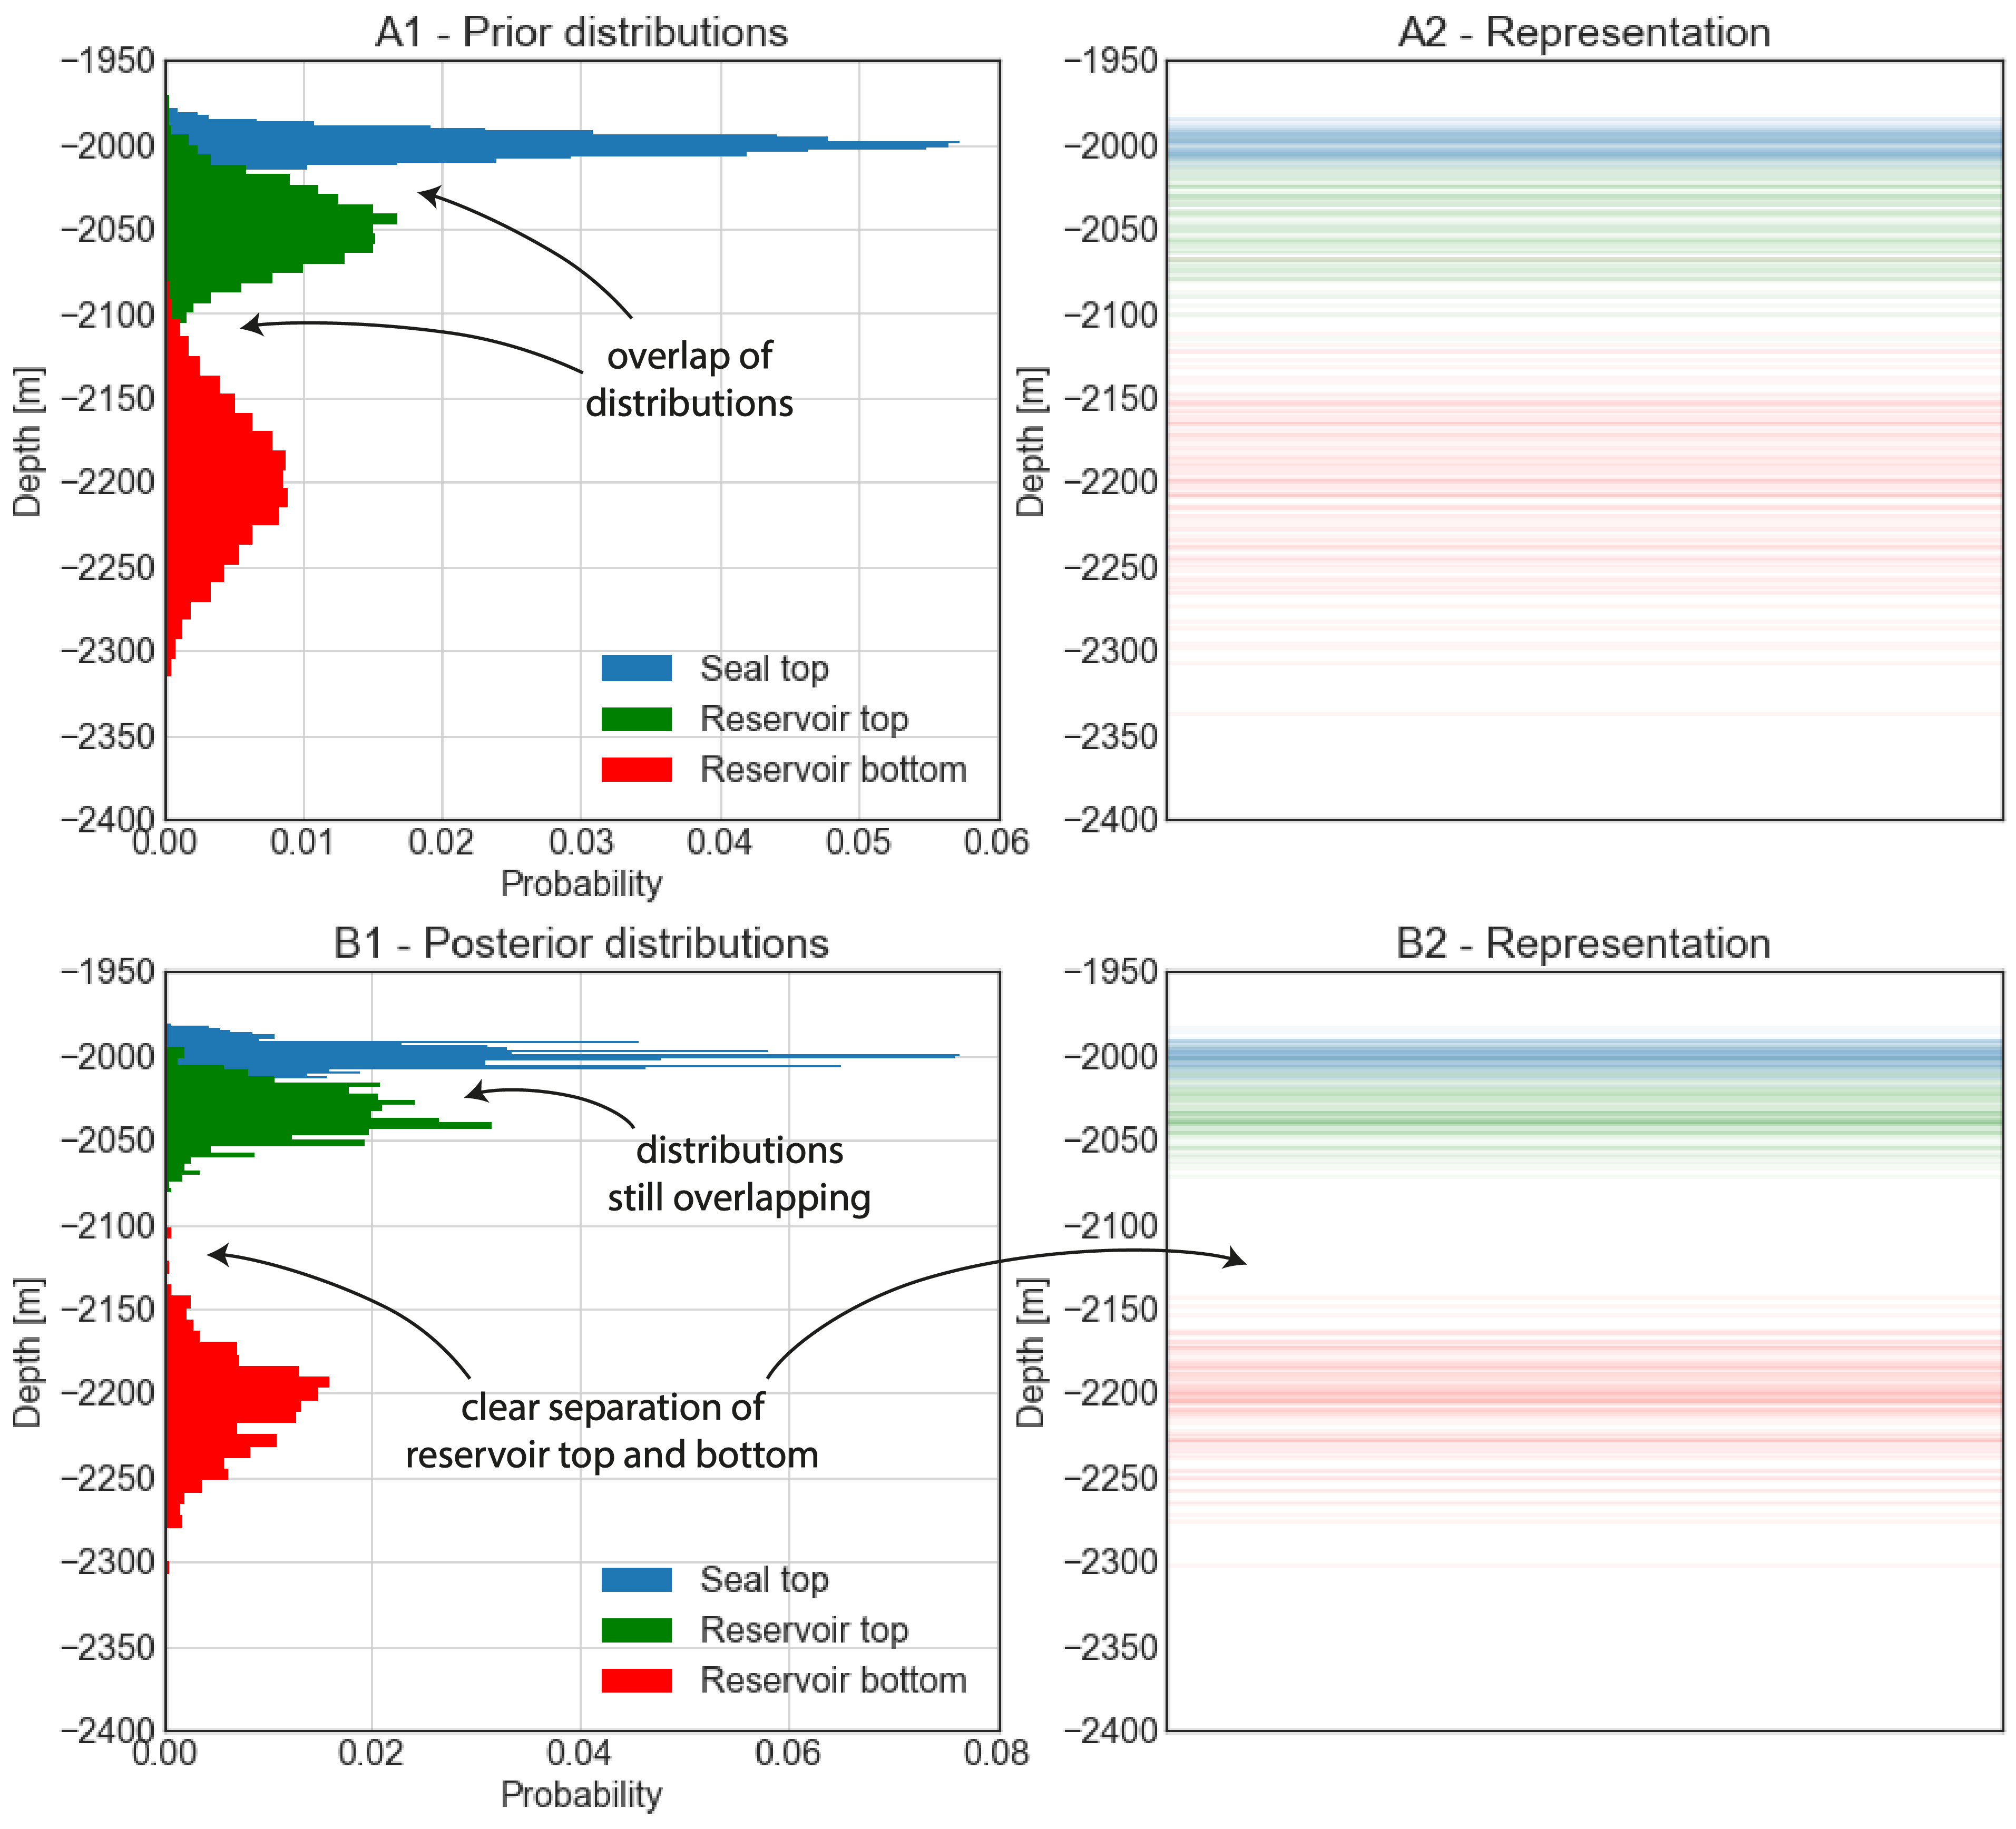
\includegraphics[width=1\textwidth]{Figures/update_moderate1.png}
				\caption{Prior (A1) and posterior distributions (A2) of the layer boundary positions in depth and respective representations (A2, B2).}\label{fig:update_moderate1} 
			\end{figure}
			
			Realizations of the four loss function adaption steps as elaborated in Section \ref{sec:LF_design} and based on the scoring results shown in Figure \ref{fig:score_results1}-B are depicted in the plots in Figure \ref{fig:LF_4steps}.
			As expected, the median is returned for the Bayes action, when using the standard symmetric absolute-error loss function (Figure \ref{fig:LF_4steps}-I). Compared to this, it can be observed that assigning a stronger weight on overestimation (Figure \ref{fig:LF_4steps}-II) steepens the curve on the right hand side and shifts the minimum to the left, i.e. to a lower estimate. Using \textit{a} = 1.25, the Bayes action changes from the median, to a value close to the mean of the distribution. The shift and steepening are significantly reinforced by the introduction of fatal overestimation (Figure \ref{fig:LF_4steps}-III). With \textit{b} = 2, the Bayes action drops to the zero score estimate. It can also be noted, that by defining a condition dependent on the algebraic sign of the values, according to which only losses for positive estimates are multiplied by \textit{b}, a distinct jump appears at the zero score boundary. Due to a similar condition, the same effect is observed on the negative side of estimate values, where the curve has also been steepened, after including fatal underestimation (Figure \ref{fig:LF_4steps}-IV). This comes with a shift of the minimum towards positive values. It is also to be noted that with every customization step, the overall expected loss is increased.\\			
			The implementation of the final custom loss function (Figure \ref{fig:LF_4steps}-IV) using single determined values for the true score is plotted in Figure \ref{fig:LF4_det_values}. This helps to clarify the way real losses result for each guess, relative to given true score values. The expected loss is acquired by arithmetically averaging such loss realizations based on the true score probability distribution by using Equation \ref{eq:ExpectedLoss2}.\\			
			Implementing risk-affinity as a factor \textit{r} leads to different steepnesses of the plotted curves depicting loss and expected loss. The effect on the latter is visualized in Figure \ref{fig:1D_LFR}, where 0.5, 0.75, 1, 1.25 and 1.5 were chosen as values for \textit{r}. 	
			It can be observed that the minima for expected loss, i.e. the Bayesian estimators for differently risk-affine actors, are located at different estimates. Mean and median are clearly surpassed by the best estimate of the most risk-friendly actor (\textit{r} = 0.5), while for the most risk-averse actors (\textit{r} = 1.25 and \textit{r} = 1.5), the Bayes action equals a zero score estimate and thus the decision to take no action. In Figure \ref{fig:1D_LFR} it can also be recognized that the expected loss is generally lower for risk-friendlier actors on the side of positive estimates, which is the relevant side for decision-making.
			
			\subsection{Bayesian updating using thickness likelihoods}
			\citet{delaVarga2016} made use of Bayesian inference to reduce the uncertainty in this type of one-dimensional model. The same is conducted here in the following.\\				
			The probability distributions for the location of the layer boundaries are treated as priors. Now it is assumed that new observations have been made, providing additional information on the likelihoods of the thicknesses of the two layers. Likelihood functions for reservoir and seal thicknesses are introduced in the form of normal distributions, defined by means and standard deviations. These parameters vary according to nature of the observations made. Using the principle of Bayesian inference as explained in Chapter \ref{sec:bayes}, the model is updated and new posterior distributions for our true reservoir score are attained\\
			Different Bayesian updating cases with different sets of likelihoods are presented in the following, so that various possible results can be compared. Each take the layer boundaries defined in Section \ref{sec:1D_construction} as priors and use Bayesian inference with respective likelihood data defined below for each case.
				
				\subsubsection{Updating case I: Moderately reinforcing information}
				\begin{figure}[h]
					\begin{subfigure}{1\textwidth}
						\centering
						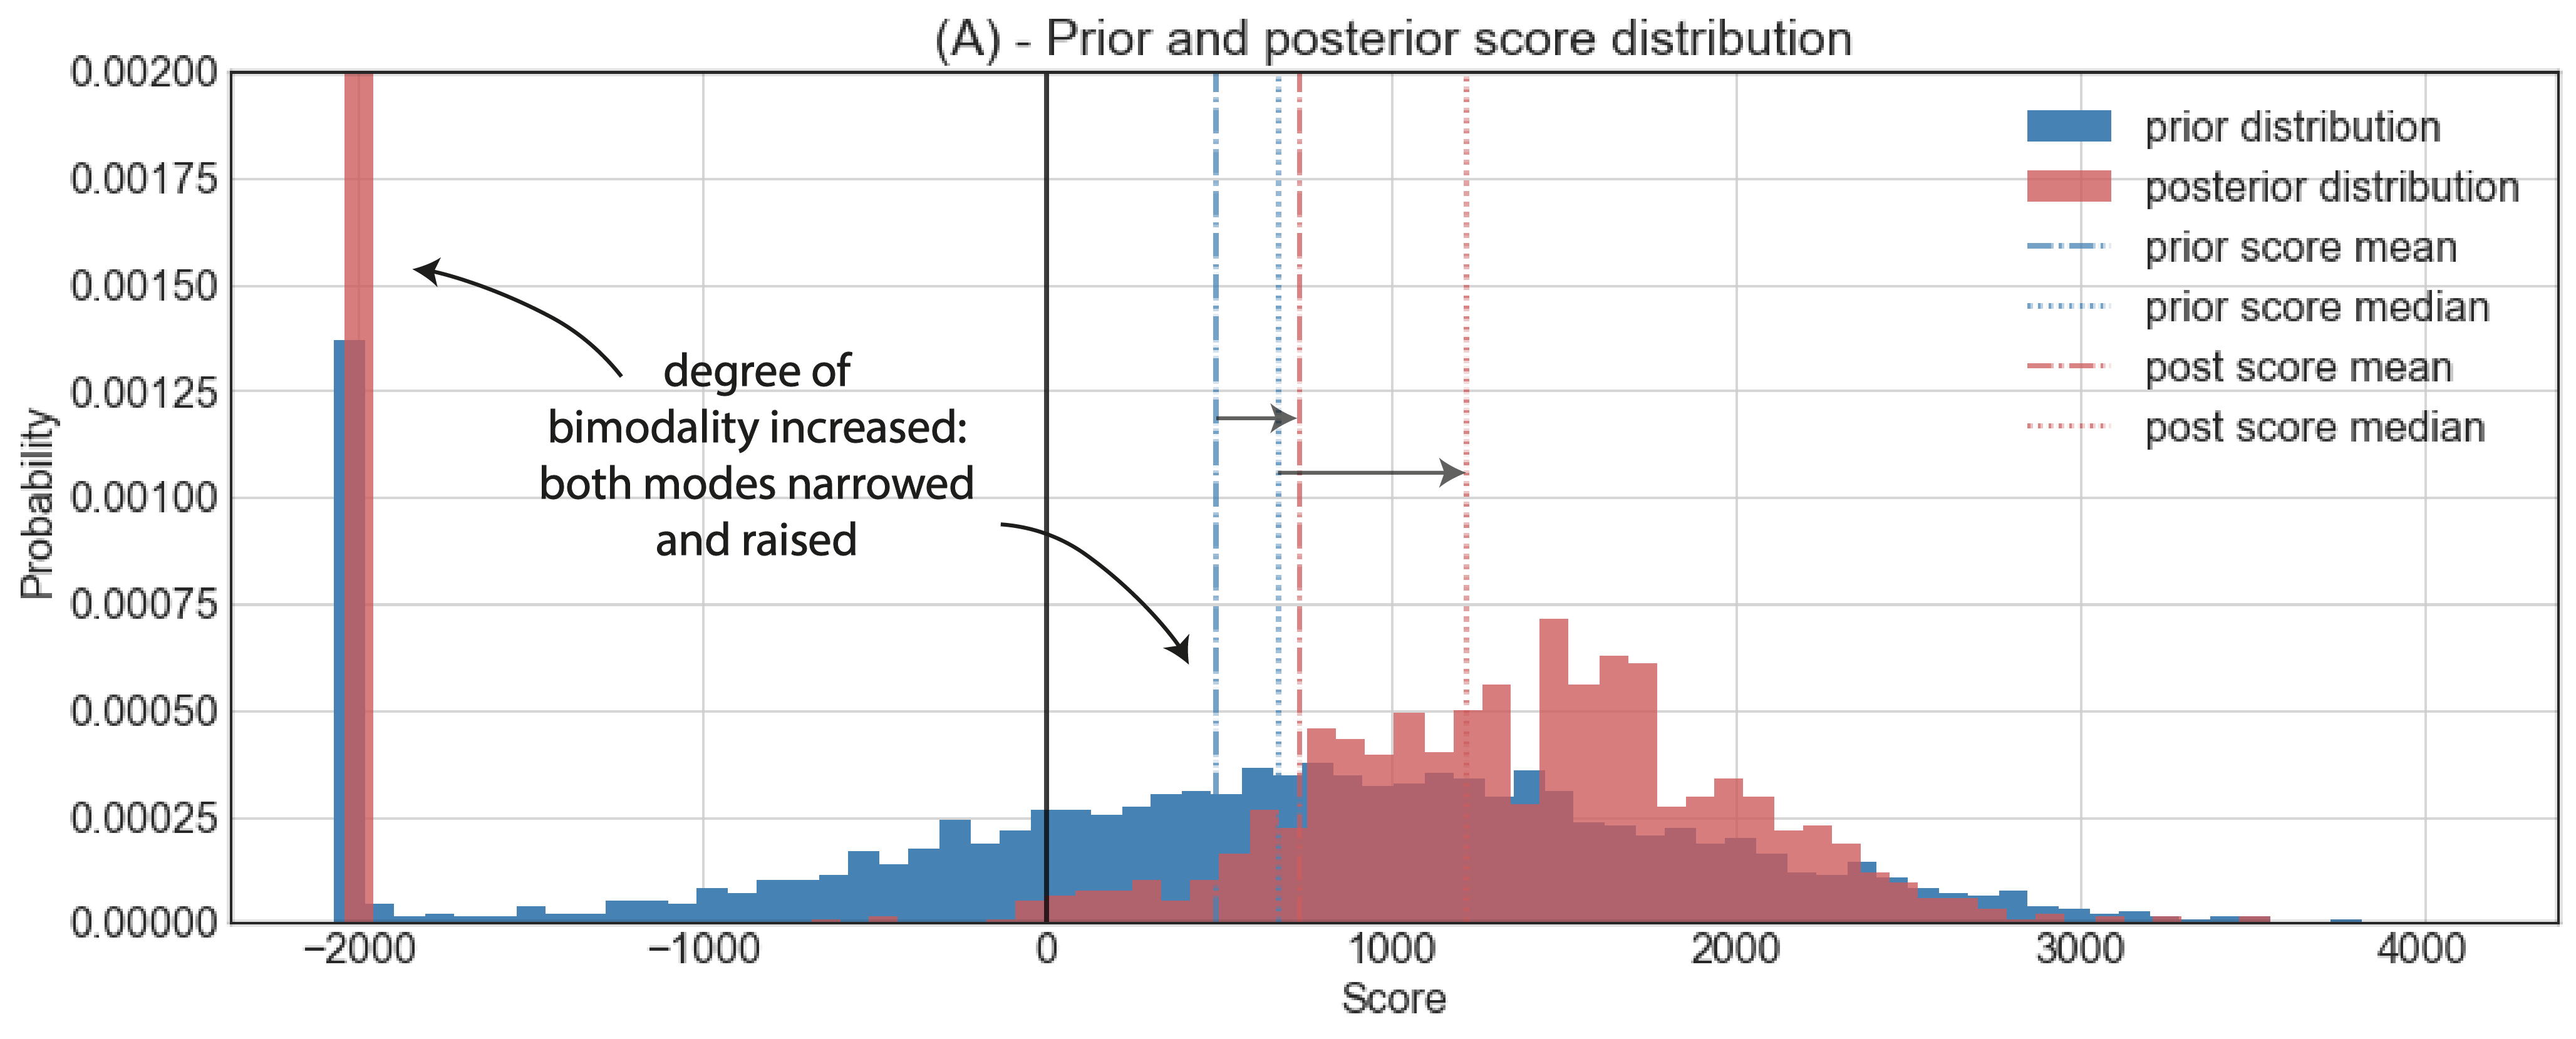
\includegraphics[width=1\linewidth]{Figures/update_moderate2.png}
						%\caption{1a}
						%\label{fig:sfig1}
					\end{subfigure}%
					\\
					\begin{subfigure}{1\textwidth}
						\centering
						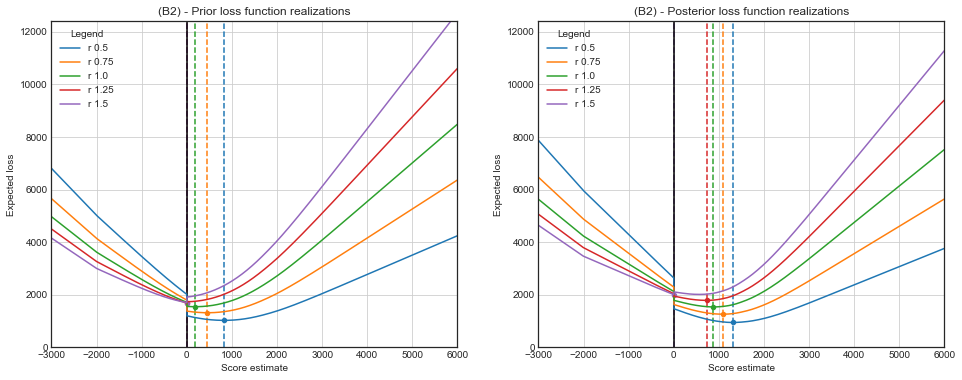
\includegraphics[width=1\linewidth]{Figures/update_moderate3.png}
						%\caption{1b}
						%\label{fig:sfig2}
					\end{subfigure}
					\caption{Reservoir score distributions (A) and change in the realizations of expected loss for several risk parameters (B1, B2) before and after Bayesian updating based on likelihoods defined as follows: Seal thickness mean = 25~m, std = 20~m. Reservoir thickness mean = 180~m, std = 60~m.}
					\label{fig:update_moderate2_3}
				\end{figure}
				
				In this first case, a normal distribution with a mean of 25~m and a standard deviation of 20~m is chosen to reflect the likelihood of the seal thickness. For the reservoir, a normal distribution with a mean of 180~m and a standard deviation of 60~m is chosen. Using these likelihoods to update the 1D geological model, the uncertainty in the posterior probability distributions for the positions of layer boundaries in depth is reduced (see Figure \ref{fig:update_moderate1}).\\					
				Scoring is applied based on these new distributions. In Figure \ref{fig:update_moderate2_3}-A, it can be recognized that the bulk of the score distribution was shifted to the positive side of values, while the peak at -2000 was raised. The probability of scores between -2000 and 0 decreased significantly, i.e. the true score is most likely either positive or -2000 if it is negative.\\
				Application of the custom loss function (Equation \ref{eq:LFR_final}) is visualized in Figure \ref{fig:update_moderate2_3}, in which the expected losses are compared before (B1) and after (B2) uncertainty reduction. It is observable, that by adding information about layer thickness likelihoods, Bayes actions are shifted relative to the nature of the information. In this case, the added data generally reinforces the probability of the reservoir to be significantly thick. Information on the seal, however, based on a normal distribution around 25~m thickness, leaves uncertainty about the reliability of the seal, as the safety threshold is defined as 20~m.\\				
				NOT INCREASED CERTAINTY; ONLY OVERALL VALUES!
				Increased certainty about the reservoir thickness is sufficient to shift Bayes actions to higher estimates for all actors, but the most risk-averse one ($r$ = 1.5). These shifts are quantified in Table \ref{tab:update_examples_all}. According to these numbers, the risk-neutral actor's estimate is increased the most, the risk-friendliest actor's estimate the least. Expected losses are decreased for the risk-neutral and the two risk-friendlier individuals. It is clear that the expected loss was reduced the most for the risk-friendliest actor and it increased most significantly for the most risk-averse actor.\\				
				%\begin{table}
				%	\centering
				%	\begin{tabular}[c]{| l | l | l |}
				%		\hline
				%		Risk factor \textit{r} & Shift in Bayes action & Change in expected loss \\ \hline
				%		0.50 & +~553.67 & -~105.49 \\ 
				%		0.75 & +~673.40 & -~81.67  \\ 
				%		1.00 & +~750.05 & -~33.56 \\ 
				%		1.25 & +~713.19 & +~75.71 \\ 
				%		1.50 & +~0.00 & +~282.64  \\ 
				%		\hline
				%	\end{tabular}
				%	\caption{Bla}
				%	\label{tab:update_moderate_tab}
				%\end{table}
								
				\subsubsection{Updating case II: Likely reliable seal}
				\begin{figure}[h]
					\begin{subfigure}{1\textwidth}
						\centering
						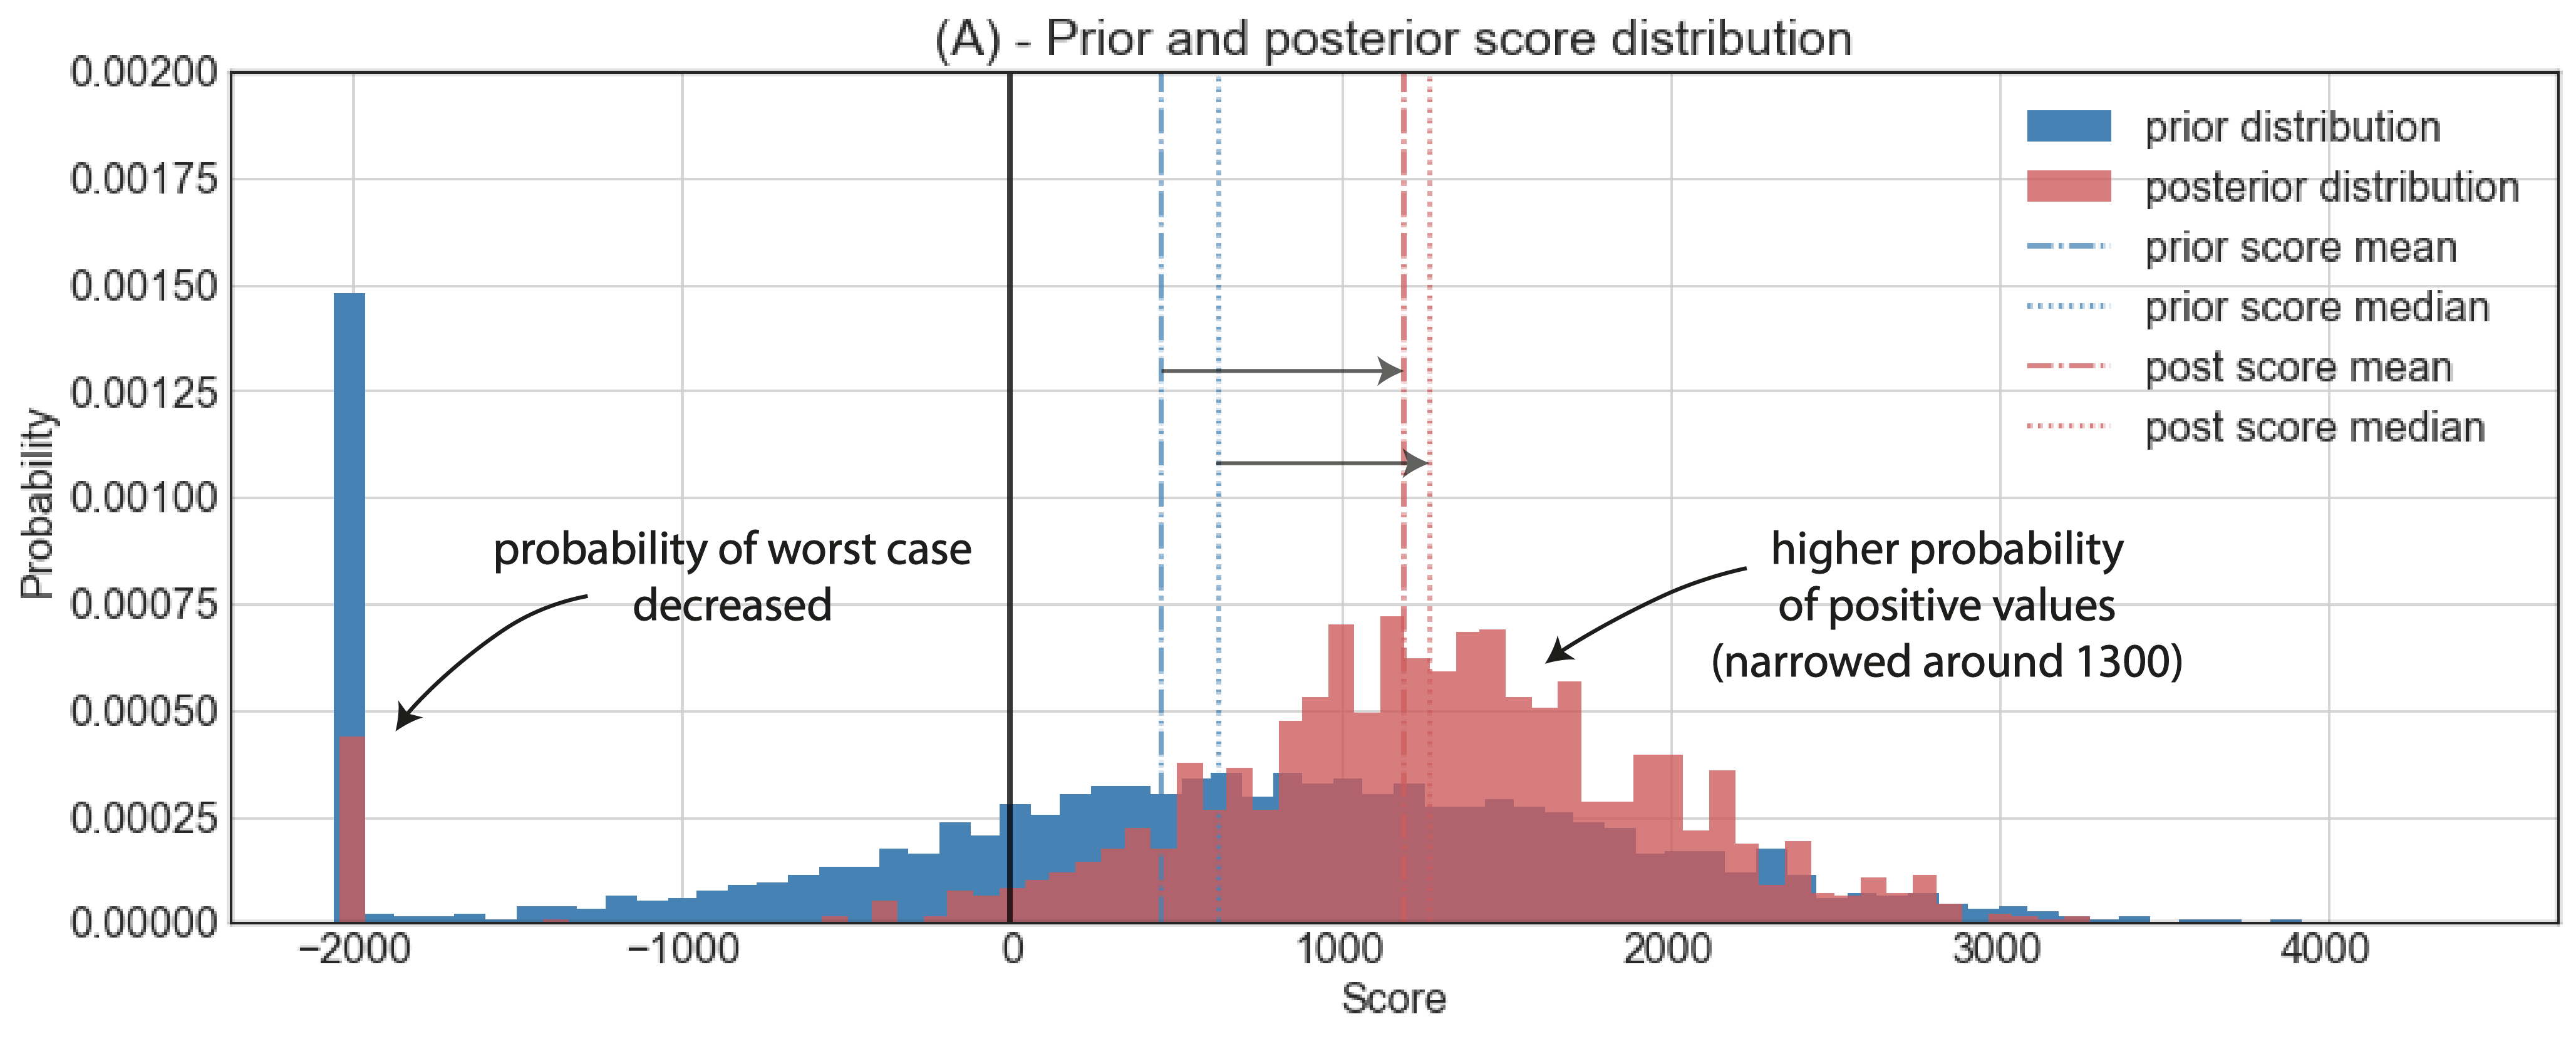
\includegraphics[width=1\linewidth]{Figures/update_goodseal2.png}
						%\caption{1a}
						%\label{fig:sfig1}
					\end{subfigure}%
					\\
					\begin{subfigure}{1\textwidth}
						\centering
						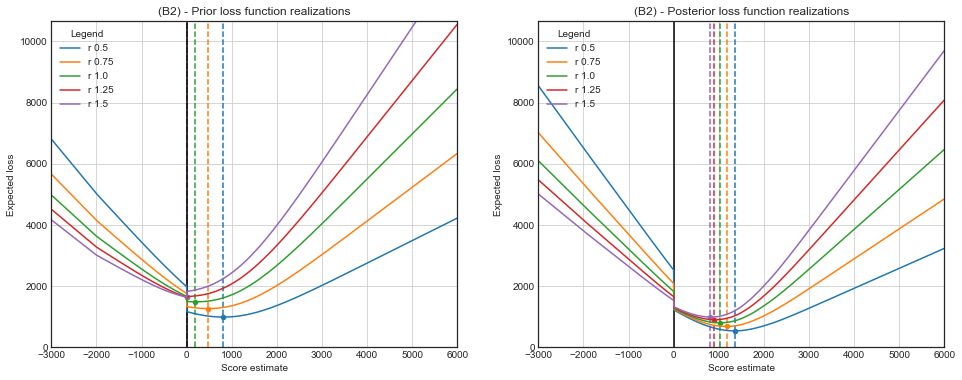
\includegraphics[width=1\linewidth]{Figures/update_goodseal3.png}
						%\caption{1b}
						%\label{fig:sfig2}
					\end{subfigure}
					\caption{Reservoir score distributions (A) and change in the realizations of expected loss for several risk parameters (B1, B2) before and after Bayesian updating based on likelihoods defined as follows: Seal thickness mean = 50~m, std = 20~m. Reservoir thickness mean = 180~m, std = 60~m.}
					\label{fig:update_goodseal2_3}
				\end{figure}
				In this second case, the reservoir thickness likelihood is defined in the same way as in case I (mean = 180~m, standard deviation = 60~m). For the seal, a mean of 50~m with a standard deviation of 20~m is chosen, favoring the likelihood of a reliable seal relative to the threshold of 20~m thickness. Respective score results are depicted in Figure \ref{fig:update_goodseal2_3}-A. The bulk of the distribution is narrowed on the positive side of estimates. Mean and median are clearly shifted to higher values. The "seal failure peak" at -2000 is significantly decreased.\\		
				Applying the custom loss function on this new score distribution results in the realizations of expected loss illustrated in Figure \ref{fig:update_goodseal2_3}. Bayes actions are shifted clearly to higher estimates and expected losses of these minima are significantly reduced for all actors. This is quantified in Table \ref{tab:update_examples_all}. According to these values, the risk-neutral to risk-averse individuals seem to profit the most, due to a large change in estimate value and decreased expected loss. Compared to case I, the estimate shifts for both risk-friendlier actors remain approximately the same, expected losses, however, are lowered much more significantly.
				POINT OUT: DECREASED UNCERTAINTY! AND HIGHER VALUES OVERALL!\\		
				%\begin{table}
				%	\centering
				%	\begin{tabular}[c]{| l | l | l |}
				%		\hline
				%		Risk factor \textit{r} & Shift in Bayes action & Change in expected loss \\ \hline
				%		0.50 & +~522.95 & -~436.26 \\ 
				%		0.75 & +~697.73 & -~551.92  \\ 
				%		1.00 & +~855.57 & -~631.92 \\ 
				%		1.25 & +~912.43 & -~647.10 \\ 
				%		1.50 & +~819.26 & -~545.96  \\ 
				%		\hline
				%	\end{tabular}
				%	\caption{Bla}
				%	\label{tab:update_goodseal_tab}
				%\end{table}
				
				\subsubsection{Updating case III: Safe seal but likely subpar reservoir thickness}
				\begin{figure}[h]
					\begin{subfigure}{1\textwidth}
						\centering
						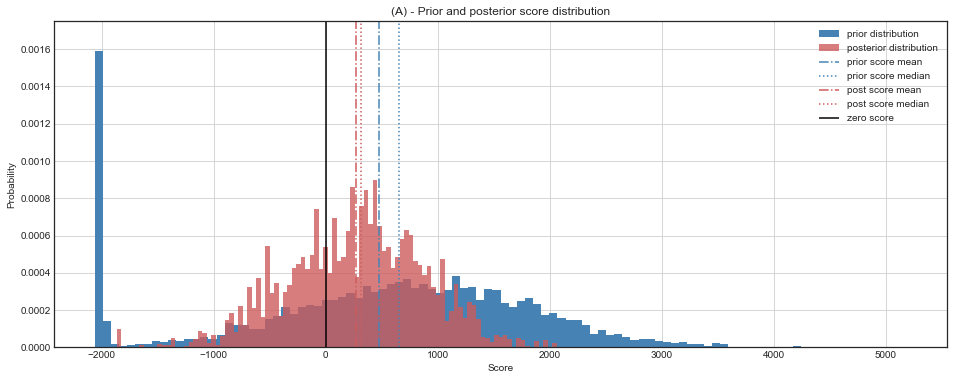
\includegraphics[width=1\linewidth]{Figures/update_smallres2.png}
						%\caption{1a}
						%\label{fig:sfig1}
					\end{subfigure}%
					\\
					\begin{subfigure}{1\textwidth}
						\centering
						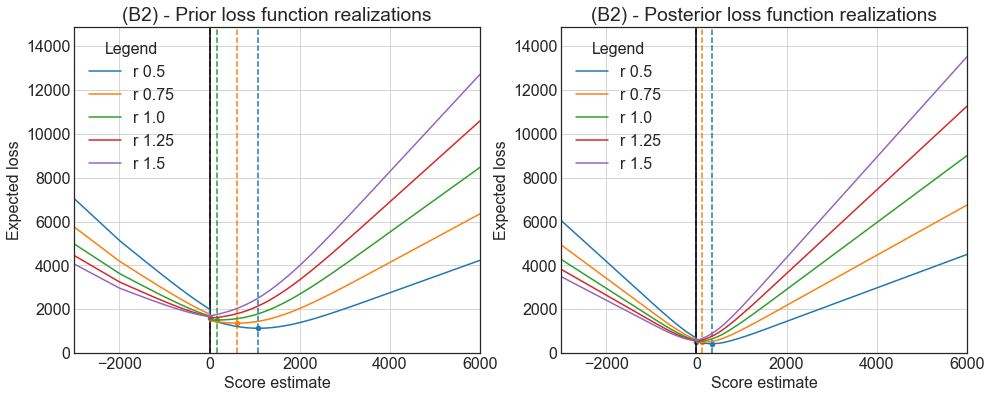
\includegraphics[width=1\linewidth]{Figures/update_smallres3.png}
						%\caption{1b}
						%\label{fig:sfig2}
					\end{subfigure}
					\caption{Reservoir score distributions (A) and change in the realizations of expected loss for several risk parameters (B1, B2) before and after Bayesian updating based on likelihoods defined as follows: Seal thickness mean = 70~m, std = 10~m. Reservoir thickness mean = 100~m, std = 40~m.}
					\label{fig:update_smallres2_3}
				\end{figure}
				In this third case, seal safety is ensured by using a mean of 70~m with a standard deviation of 10~m for the seal thickness likelihood. However, the new observations are assumed to provide information about the reservoir unit that makes it likely to be thinner than expected. Reservoir thickness likelihood is assigned a mean of 100~m and a standard deviation of 40~m.\\				
				The subsequent score distribution is depicted in Figure \ref{fig:update_smallres2_3}. It can be seen that while the whole distribution is narrowed, it also is shifted to the left, to lower and negative estimates. Mean and median are almost the same. As seal reliability is practically guaranteed, the peak at -2000~m vanishes.\\				
				Based on this reservoir score probability distribution, Bayes actions are shifted to lower estimates for all actors using the custom loss function (see Figure \ref{fig:update_smallres2_3}). In fact, all but the most risk-friendly individual (\textit{r}~=~0.5) find their Bayesian estimator to be zero now, i.e. project development is deemed to be too risky to them. Furthermore, the spread of expected loss values around the minima for all actors is diminished. In other words, the expected loss values of the Bayes actions are now much closer to each other. Notable is the large reduction of expected loss in general. Quantified changes in the positions and values of the Bayes actions are listed in Table \ref{tab:update_examples_all}. There is no shift in estimate for risk-averse actors, as they already found their best estimates to be zero before updating.
				DECREASED UNCERTAINTY BUT AT THE SAME TIME LOWER VALUES OVERALL!\\
				%\begin{table}
				%	\centering
				%	\begin{tabular}[c]{| l | l | l |}
				%		\hline
				%		Risk factor \textit{r} & Shift in Bayes action & Change in expected loss \\ \hline
				%		0.50 & -~498.98 & -~538.08 \\ 
				%		0.75 & -~346.16 & -~717.83  \\ 
				%		1.00 & -~176.13 & -~872.02 \\ 
				%		1.25 & -~0.00 & -~946.04 \\ 
				%		1.50 & -~0.00 & -~951.57  \\ 
				%		\hline
				%	\end{tabular}
				%	\caption{Bla}
				%	\label{tab:update_smallres_tab}
				%\end{table}
				
				\begin{table}
					\centering
					\begin{tabular}[c]{| c || l | l || l | l || l | l |}
						\hline
						& Example I & & Example II & & Example III & \\
						\hline
						\hline
						\textit{r} & $\Delta$ BA & $\Delta$ EL & $\Delta$ BA & $\Delta$ EL & $\Delta$ BA & $\Delta$ EL\\ 
						\hline
						0.50 & +~553.67 & -~105.49 & +~522.95 & -~436.26 & -~498.98 & -~538.08 \\ 
						0.75 & +~673.40 & -~81.67 & +~697.73 & -~551.92 & -~346.16 & -~717.83  \\ 
						1.00 & +~750.05 & -~33.56 & +~855.57 & -~631.92 & -~176.13 & -~872.02 \\ 
						1.25 & +~713.19 & +~75.71 & +~912.43 & -~647.10 & -~0.00 & -~946.04 \\ 
						1.50 & +~0.00 & +~282.64 & +~819.26 & -~545.96 & -~0.00 & -~951.57  \\ 
						\hline
					\end{tabular}
					\caption{Changes in Bayes action (BA) and minimal expected loss (EL) for Bayesian updating cases I, II and III and respective actors with risk parameters $r$.}
					\label{tab:update_examples_all}
				\end{table}
				%\begin{table}
				%		\begin{tabular}[c]{| l | l | l |}
				%			\hline
				%			Risk factor \textit{r} & Shift in Bayes action & Change in expected loss \\ \hline
				%			0.50 & -~498.98 & -~538.08 \\ 
				%			0.75 & -~346.16 & -~717.83  \\ 
				%			1.00 & -~176.13 & -~872.02 \\ 
				%			1.25 & -~0.00 & -~946.04 \\ 
				%			1.50 & -~0.00 & -~951.57  \\ 
				%			\hline
				%		\end{tabular}
				%		\caption{Bla}
				%		\label{tab:update_examples_all}
				%\end{table}
				
				NEED TO INCLUDE CLEAR BA VALUES BEFORE AND AFTER!!! NOT VISIBLE IN PLOTS.
				
			\subsection{General 1D model updating results}
			It is already shown by these three abstract 1D modeling cases, how Bayesian updating and change in uncertainties affects the way differently risk-affine decision-makers choose best estimates based on the custom loss function (Equation \ref{eq:LFR_final}). As can be expected intuitively, reassurance of positive scores, for example by narrowing of the distribution of scores on the side of positive estimates or by reducing the occurrence of negative extrema, leads to shifts towards higher Bayes action estimates for all actors. Conversely, actors are discouraged to expect gains when facing a higher probability of negative scores. Unsurprising is also the inverse behavior of risk-averse and risk-friendly individuals. However, it is most notable that a reduction of uncertainty in any case leads to a diminished spread of Bayes actions between all actors. In other words, given better information about the true value of the reservoir, different actors come to more similar decisions. Given perfect information, all actors would presumably choose the same estimate, which would equal the true score.
				
		\section{Results using the 3D geological model}
		